\section{介绍}

\subsection{\TeX 排版系统历史}

\begin{frame}[fragile]{\TeX 与 \LaTeX{} 的起源}
  \begin{columns}[T]
    % \hspace{-2em}
    \column{.9\textwidth}
    \begin{itemize}
      \item \TeX: $\tau\varepsilon\chi$ (\textipa{/'tEx/},
        \textipa{/'tEk/})
        \begin{itemize}
          \item 生成精美图书的排版系统
          \item 最初由 高德纳\footnote{1974年图灵奖得主,《计算机程序设计艺术》(The Art of Computer Programming)作者。} (Donald E.~Knuth) 于 1978 年开发  
          \item 最新版本为 \TeX\ 3.141592653
          \item 漂亮、美观、稳定、通用
          \item 尤其擅长数学公式排版
        \end{itemize}
        \vspace{2em}
      \item \LaTeX{}(\textipa{/'la:tEx/}, \textipa{/'leItEk/})
        \begin{itemize}
          \item Leslie Lamport\footnote{2013年图灵奖得主,对于分布式及并行系统的理论与实践具有基础性贡献。} 开发的一种 \TeX 格式
          \item 在 \TeX 的基础上提供宏包, 降低使用门槛
          \item 极其丰富的宏包,提供扩展功能
          \item 广泛用于学术界,期刊会议论文模板
        \end{itemize}
    \end{itemize}
    \column{.2\textwidth}
    \vspace*{-5mm}
    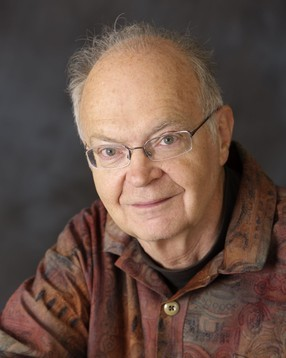
\includegraphics[width=\textwidth]{Knuth.jpg}

    % \vspace*{5mm}
    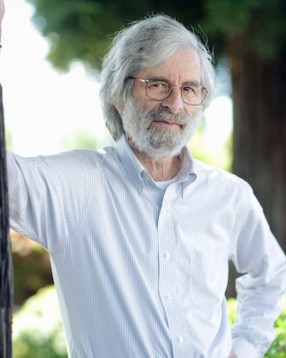
\includegraphics[width=\textwidth]{Lamport.jpg}

  \end{columns}
\end{frame}

\subsection{\LaTeX{} 利弊}

\begin{frame}[fragile]{为什么是\LaTeX{}?}
\textbf{你真的需要\LaTeX{}吗?}

\begin{itemize}
  \item \textbf{预设定的模板?}
  \begin{itemize}
    \item Word同样可以制定各种文档模板
  \end{itemize}
  \item \textbf{数学公式输入?}
  \begin{itemize}
    \item Word自带的公式功能在大多数情况下是足够使用的
    \item MathType插件可以实现高质量的公式编辑
  \end{itemize}
  \item \textbf{文献与图表公式的交叉引用?}
  \begin{itemize}
    \item 通过文献管理软件,Word同样可以方便地进行文献引用
    \item Word同样可以快捷实现对图表的交叉引用
  \end{itemize}
\end{itemize}

\end{frame}

\begin{frame}[fragile]{为什么是\LaTeX{}?}
  \textbf{为什么还要选择\LaTeX{}?}
  
  \begin{itemize}
    \item \textbf{更加流畅的编辑体验}
    \begin{itemize}
      \item Word中的内容和排版是混合的,更新内容需要同步更新排版
      \item 长达数十页且包含大量超链接和域的Word文档编辑会变得卡顿
    \end{itemize}
    \item \textbf{更加优雅的公式排版}
    \begin{itemize}
      \item \LaTeX{}相比于Word原生公式提供了更加丰富的对齐、排版功能
      \item 无需引入额外的插件
    \end{itemize}
    \item \textbf{更加省心的格式控制}
    \begin{itemize}
      \item 内容与格式分离,可以专注于内容的书写
      \item 对于图表公式的交叉引用提供了统一格式,更加便捷
    \end{itemize}
  \end{itemize}
  \end{frame}

\begin{frame}[fragile]{\LaTeX{} 的好处与坏处}
    \textbf{好处}
    \begin{itemize}
        \item 数学公式排版优雅 \quad $\mathcal{F}(\xi)=\int_{-\infty}^{\infty} f(x)\mathrm{e}^{-\mathrm{j}2\pi \xi x}\,\mathrm{d}x$
        \item 内容与格式分离
        \item 随心所欲的宏定义与自定义命令 \rawcmd{\textbackslash newcommand},\rawcmd{\textbackslash def}
    \end{itemize}

    \vspace{2em}
    \textbf{坏处}
    \begin{itemize}
        \item 得到易读的版本,需要编译
        \item 输入相对 Word 繁琐
        \item 非开箱即用。有时需要自行解决编辑器、宏包,甚至是编译错误。
    \end{itemize}
\end{frame}

\subsection{\LaTeX{}编写流程}
\begin{frame}[fragile]{怎样使用\LaTeX{}得到一个PDF?}
	\begin{enumerate}
		\item 选择/编写 \LaTeX{}模板
		      \begin{itemize}
			      \item 通常直接下载给定的\LaTeX{}模板即可
		      \end{itemize}
		\item 编写文档内容
		      \begin{itemize}
			      \item 导入需要使用的包(可选)
			      \item 按\LaTeX{}语法组织内容,编写\LaTeX{}源文件
		      \end{itemize}
		\item 编译文件
		      \begin{itemize}
			      \item 使用\XeLaTeX{}等编译器对源文件进行编译
		      \end{itemize}
    \item \alert{对照格式要求,检查最终的文件}
	\end{enumerate}
\end{frame}
